\documentclass[10pt]{beamer}
\usetheme{default}
\setbeamercovered{invisible}
\setbeamertemplate{navigation symbols}{}
\setbeamertemplate{footline}{
    \flushright{\hfill \insertframenumber{}/\inserttotalframenumber}
}

\begin{document}
    \title{Contagion:\\a discrete SIR epidemiological model}
    \author{Pasquale Claudio Africa}
    \date{26/03/2020}
    
\begin{frame}[plain, noframenumbering]
    \maketitle
\end{frame}

\begin{frame}{Contagion model\footnote{This exercise is inspired by models shown in \\
\url{https://www.washingtonpost.com/graphics/2020/world/corona-simulator/} and \\
\url{https://github.com/seismotologist/coronaVirusContagion}.}}

Consider a discrete population of people living in a 2D square domain.

\begin{figure}
    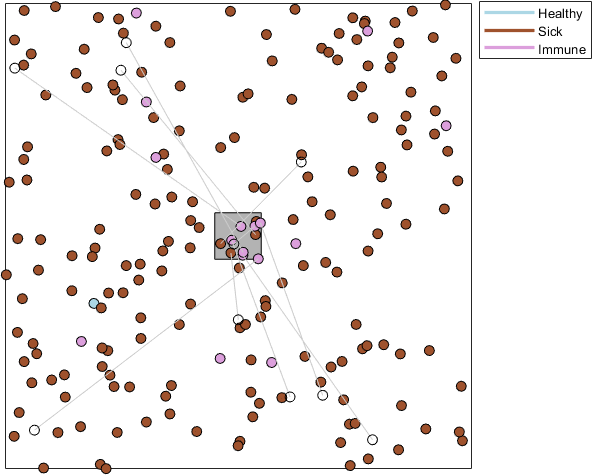
\includegraphics[width=0.75\textwidth]{contagion.png}
\end{figure}
\end{frame}

\begin{frame}{Contagion model}
Starting from random initial positions, the population evolves according to the following rules:

\begin{itemize}
    \item each person can be either Susceptible to a virus, Infected or Recovered;
    \item at each timestep people move randomly of a given step length;
    \item a prescribed percentage of people does \textbf{social distancing}, \textit{i.e.} does not move, excepted the following rule;
    \item each person (\textit{i.e.} including those who do social distancing) goes to a pub placed at the center of the domain once every a fixed number of time steps;
    \item a person is infected when close to another infected person and recovers after a fixed number of time steps.
\end{itemize}
\pause
Implement a \texttt{C++} program that
\begin{enumerate}
    \item reads all the parameters from an input file;
    \item performs the simulation;
    \item exports the total number of susceptible, infected and recovered people at each timestep to a \texttt{.csv} file;
    \item plots the solution using \texttt{gnuplot-iostream}\\
          (requires \texttt{Boost} and \href{http://www.gnuplot.info/download.html}{\texttt{gnuplot}}).
\end{enumerate}
\end{frame}

\begin{frame}{Possible extensions (homework)}
\begin{itemize}
    \item Personalize person-specific parameters, \textit{e.g.}
    \begin{itemize}
        \item by random generation;
        \item by reading multiple pairs of \{person index, parameter value\}\\
              for each parameter from file;
    \end{itemize}
    \item Take into account for birth and mortality rates.
    \item Extend the model to 3D domains (possibly using templates).
\end{itemize}
\end{frame}
\end{document}
